\documentclass[a4paper,11pt,titlepage]{article}

%Εισαγωγή γλωσσικής υποστήριξης
%ελληνικό hyphenation

\usepackage[cm-default]{fontspec}
\usepackage{xunicode}
\usepackage{xltxtra}
\usepackage{xgreek}
\usepackage[colorlinks]{hyperref}
\usepackage{enumerate}
\usepackage{amsmath}
\usepackage{float} %Places the float at precisely the location in the LaTeX code.
%η γραμματοσειρά
%\setmainfont[Mapping=tex-text]{Times New Roman} %απλοποιημένο σε σχέση με το άρθρο
\setmainfont[Mapping=tex-text]{Linux Libertine}
\newcommand{\degrees}{^{\circ}}
%page orientation
\usepackage{a4wide}
\voffset = -0.5in
\textheight = 664pt

%Άλλα χρήσιμα πακέτα
\usepackage{graphicx} 	%εισαγωγή εικόνων jpg/png κλπ
\usepackage{listings}
\lstset
{
commentstyle=\textit,
captionpos=b,
breakatwhitespace=true,
showstringspaces=false,
breaklines=true,
keywordstyle=\color{black}\bfseries,
float=htb,
frame=single
}

%απενεργοποίηση του indent στις νέες παραγράφους
\parindent=0in

%macro που δίνει το μέγιστο επιτρεπτό μέγεθος σε μια εικόνα χωρίς να παραβιάζει τα όρια του LaTeX
\makeatletter
\def\maxwidth{
\ifdim\Gin@nat@width>\linewidth
\linewidth
\else
\Gin@nat@width
\fi
    }
\makeatother

\title{1η Άσκηση\\kn}
\author{Axil}
\date{\today}

\begin{document}

\pagestyle{headings}    %αρίθμηση στο πάνω μέρος της σελίδας

%\maketitle
\begin{titlepage}
\begin{center}

\includegraphics[width=50mm]{pyrforos.pdf}\\[0.5cm]
\textbf{\LARGE ΕΘΝΙΚΟ ΜΕΤΣΟΒΙΟ ΠΟΛΥΤΕΧΝΕΙΟ}\\
\textrm{\Large Σχολή Εφαρμοσμένων Μαθηματικών και Φυσικών Επιστημών}\\[2.0cm]
\Huge{Εργαστήριο Οπτοηλεκτρονικής}\\
\Large{\textit{7o εξάμηνο, ΣΕΜΦΕ}}\\[2.0cm]
\Large{\textit{\textbf{Ηλεκτροοπτικό φαινόμενο Pockels}\\Προσδιορισμός τάσης $V_{\lambda /4}$ κρυστάλλου KDP}}\\[5.0cm]
\normalsize
\begin{minipage}{0.49\textwidth}
\begin{flushleft}
\textbf{Πιπινέλλης Αχιλλέας}, 09103163
\end{flushleft}
\end{minipage}
\begin{minipage}{0.49\textwidth}
\begin{flushright}
\textbf{\textit{Η/Μ Παράδοσης:} 20 Ιανουαρίου 2012}
\end{flushright}
\end{minipage}
%\maketitle

\vfill
%bottom of the page
{Αθήνα, 2012}

\end{center}
\end{titlepage}

%\maketitle

\section{Θεωρία}

\subsection{Εισαγωγή}

Στην παρούσα άσκηση θα μελετήσουμε το διαμήκες γραμμικό ηλεκτροοπτικό φαινόμενο σε θερμοκρασία περιβάλλοντος για κρυστάλλους KDP. Θα προσδιορίσουμε την τάση $V_{\lambda/4}$ η οποία εφαρμοζόμενη σε κατάλληλα προσανατολισμένο ηλεκτροοπτικό κρύσταλλο προκαλεί στις δύο συνιστώσες της φωτεινής δέσμης διαφορά φάσης ίση με $\pi /2$. Το φαινόμενο αυτό είναι γνωστό και ως φαινόμενο Pockels.

\subsection{Ηλεκτροοπτικό Φαινόμενο}

Όταν σε ένα οπτικό μέσο εφαρμοστεί εξωτερικό ηλεκτρικό πεδίο, οι τροχιές των ηλεκτρονίων στα άτομα του υλικού διαταράσσονται, με αποτέλεσμα τη μεταβολή των οπτικών του χαρακτηριστικών, όπως για παράδειγμα ο δείκτης διάθλασης. Η εφαρμογή εξωτερικού ηλεκτρικού πεδίου σε ορισμένους κρυστάλλους προκαλεί φαινόμενα διπλοθλαστικότητας. Διπλοθλαστικότητα είναι η διάσπαση μιας ακτίνας φωτός (και άλλης Η/Μ ακτινοβολίας) σε δύο ακτίνες (τακτική και έκτακτη) όταν περνάει μέσα από συγκεκριμένους τύπους υλικών, και βασίζεται στην πόλωση του φωτός. Για παράδειγμα, η εφαρμογή ενός εξωτερικού πεδίου σε ένα οπτικά ισότροπο κρύσταλλο (δηλαδή σε υλικό που διατηρεί τον ίδιο δείκτη διάθλασης προς όλες τις διευθύνσεις), μπορεί να μεταβάλλει τη διηλεκτρική του πόλωση και να τον μετατρέψει σε διπλοθλαστικό (οπτικά ανισότροπο), με μικρές μεταβολές του δείκτη διάθλασης. Το φαινόμενο αυτό είναι γνωστό ως ηλεκτροοπτικό φαινόμενο.\\
Αν θεωρήσουμε το δείκτη διάθλασης $n$ ως συνάρτηση του εφαρμοζόμενου ηλεκτρικού πεδίου, δηλαδή $n = n(E)$, τότε\\[7pt]
$n(E) = n_0 + a_1 E + \frac{1}{2} a_2 E^2 + ...$ (σειρά Taylor ως προς Ε) (1)\\[7pt]
όπου ο συντελεστής $a_1$ καλείται συντελεστής γραμμικού ηλεκτροοπτικού φαινομένου και ο συντελεστής $a_2$ καλείται συντελεστής δευτέρου βαθμού ηλεκτροοπτικού φαινομένου. Η μεταβολή του δείκτη διάθλασης $n$, εξ αιτίας του πρώτου όρου $E$ καλείται φαινόμενο Pockels, ενώ η μεταβολή του εξ' αιτίας του δεύτερου όρου $E^2$ καλείται φαινόμενο Kerr και επομένως τα δυο φαινόμενα διαμορφώνονται ως:\\[7pt]
$\Delta n = a_1 E $ (φαινόμενο Pockels) (2)\\[7pt]
$\Delta n = a_2 E^2 = (\lambda K) E^2 $ (φαινόμενο Kerr) (3) \\[7pt]
όπου $\lambda$ το μήκος κύματος της προσπίπτουσας ακτινοβολίας και Κ ο συντελεστής Kerr. Εδώ να σημειώσουμε ότι το φαινόμενο Pockels το παρουσιάζουν μόνο μερικά κρυσταλλικά υλικά, ενώ το φαινόμενο Kerr το παρουσιάζουν όλα τα υλικά.
\newpage
\subsection{Φαινόμενο Pockels}

Το 1906 ο Γερμανός φυσικός Friedrich Pockels περιέγραψε πρώτος το ηλεκτροοπτικό φαινόμενο που παρατηρείται σε ορισμένους κρυστάλλους όπως το δισόξινο φωσφορικό κάλιο ($KH_2PO_4$ συντομογραφικά: KDP). Διαφέρει από το φαινόμενο Kerr κατά το ότι το φαινόμενο Pockels είναι γραμμικό ως προς το εφαρμοζόμενο ηλεκτρικό πεδίο, ενώ το φαινόμενο Kerr, όπως είδαμε είναι ανάλογο του τετραγώνου του εφαρμοζόμενου ηλεκτρικού πεδίου.\\
Μία κυψελίδα Pockels (Σχήμα 1) είναι μία συσκευή η οποία αποτελείται από έναν ηλεκτροοπτικό κρύσταλλο (με μερικά ηλεκτρόδια συνδεδεμένα πάνω του) μέσω του οποίου μπορεί να διαδοθεί μια φωτεινή δέσμη. Ας υποθέσουμε ότι μια κυψελίδα Pockels κατεσκευάζεται με εφαρμογή ενός ηλεκτρικού πεδίου σ' έναν κρύσταλλο, όπως ο KDP, παράλληλα προς τον οπτικό άξονά του. Η διεύθυνση διάδοσης της φωτεινής δέσμης είναι επίσης παράλληλη προς τον οπτικό άξονα. Όταν δεν υπάρχει ηλεκτρικό πεδίο, κάθε ακτίνα που διαδίδεται σε διεύθυνση παράλληλη προς τον οπτικό άξονα, είναι μία τακτική ακτίνα και ο δείκτης διάθλασης είναι ανεξάρτητος της διεύθυνσης πόλωσης.\\
Το ηλεκτρικό πεδίο παραμορφώνει τον κρύσταλλο και επάγει ένα δεύτερο οπτικό άξονα $OA'$ στο επίπεδο κάθετο στο πεδίο. Η διεύθυνση του $OA'$ εξαρτάται από τη δομή του κρυστάλλου. Λόγω της πρόσθετης ανισοτροπίας που επάγεται από το ηλεκτρικό πεδίο, ακτίνες που είναι πολωμένες με τα διανύσματα των ηλεκτρικών τους πεδίων παράλληλα προς τον $OA'$ αντιμετωπίζουν ένα δείκτη διάθλασης που διαφέρει από αυτόν των ακτίνων που είναι πολωμένες κάθετα προς το $OA'$. Δηλαδή, όταν εφαρμόζεται ηλεκτρικό πεδίο, ο κρύσταλος λειτουργεί πάνω στη φωτεινή ακτίνα σαν διπλοθαστικός κρύσταλλος του οποίου ο άξονας κείται στο επίπεδο το κάθετο προς τη διεύθυνση διάδοσης. \\
Η διαφορά μεταξύ των δεικτών διάθλασης για ακτίνες πολωμένες κάθετα και παράλληλα προς το $OA'$ είναι \\[7pt]
$(n_0-n_e)' = pE$\\[7pt]
όπου $E$ είναι το εφαρμοζόμενο πεδίο και το $p$ είναι μία σταθερά αναλογίας. Το $p$ είναι περίπου ίσο με $3.6\times 10^{-11}m.V^{-1}$ για το KDP που θα μελετήσουμε.\\
Επειδή το πεδίο εφαρμόζεται παράλληλα προς τον οπτικό άξονα, η προηγούμενη περίπτωση είναι γνωστή και ως διαμήκες φαινόμενο Pockels.
\begin{figure} [bph!]
\centering
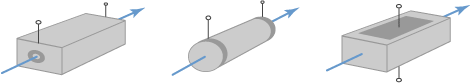
\includegraphics[width=100mm]{pockels_cells.png}
\caption{Κυψελίδες Pockels}
\end{figure}


\newpage
\subsection{Κυκλικά πολωμένο φως}
\subsubsection{Θεωρία}
Κυκλική πόλωση ενός Η/Μ κύματος είναι η πόλωση όπου το διάνυσμα του ηλεκτρικού πεδίου, σε κάποιο συγκεκριμένο σημείο στο χώρο, περιγράφει ένα κύκλο καθώς ο χρόνος προχωρά. Αν παγώσουμε το κύμα στο χρόνο, το διάνυσμα του ηλεκτρικού πεδίου περιγράφει μία έλικα προς τη διεύθυνση της διάδοσης. Η κυκλική πόλωση είναι μια ειδική περίπτωση της ελλειπτικής πόλωσης. Για να εισάγουμε την έννοια της κυκλικής πόλωσης, ας υποθέσουμε ότι δύο γραμμικά πολωμένα κύματα που διαδίδονται στους άξονες $y$ και $z$ αντίστοιχα, είναι σε φάση και έχουν ίσα πλάτη. Αν θεωρήσουμε την επαλληλία τους, κάθε σημείο τους υφίσταται ταυτόχρονες μετατοπίσεις κατά μήκος των διευθύνσεων $y$ και $z$ που έχουν το ίδιο μέτρο. Το προκύπτον συνιστάμενο κύμα κείται επί επιπέδου που σχηματίζει γωνία $45\degrees$ με τους άξονες $y$ και $z$ (δηλαδή επί επιπέδου που σχηματίζει γωνία $45\degrees$ με τα επίπεδα $xy$ και $xz$). Το πλάτος του συνιστάμενου κύματος είναι μεγαλύτερο κατά τον παράγοντα $\sqrt[]{2}$ από το πλάτος του καθενός επιμέρους συνιστώντος κύματος, ενώ το συνιστάμενο κύμα είναι γραμμικώς πολωμένο. \\ 
Ας υποθέσουμε τώρα ότι τα δύο κύματα ίσου πλάτους έχουν διαφορά φάσης $\pi/2$, που ισοδυναμεί με διαφορά φάσης τεταρτοκυκλίου. Σ'αυτή την περίπτωση η συνιστάμενη κίνηση κάθε σημείου περιγράφεται από μια υπέρθεση δύο απλών αρμονικών κινήσεων κατά μήκος δύο κάθετων αξόνων, ενώ η διαφορά φάσης τους είναι $\pi/2$, που αντιστοιχεί σε διαφορά φάσης τεταρτοκυκλίου. Η μετατόπιση $y$ ενός σημείου είναι μέγιστη τη χρονική στιγμή κατά την οποία η μετόπιση $z$ είναι μηδέν και αντιστρόφως. Συνεχόμενα σημεία των κυμάτων έχουν διαδοχικές διαφορές φάσεις, με αποτέλεσμα η συνολική κίνηση να έχει τη μορφή μιας περιστρεφόμενης έλικας. Αυτή η συγκεκριμένη υπέρθεση δύο γραμμικώς πολωμένων κυμάτων ονομάζεται {\bf κυκλική πόλωση}. Συμβατικά λέμε ότι το κύμα είναι κυκλικά πολωμένο δεξιόστροφα (Σχήμα 2), αν η φορά κίνησης $-$ για ένα παρατηρητή με κατεύθυνση παρατήρησης \textit{από εμπρός προς τα πίσω} και κατά μήκος της κατεύθυνσης διάδοσης $-$ \textit{συμπίπτει με τη φορά των δεικτών του ρολογιού}.
\begin{figure} [bph!]
\centering
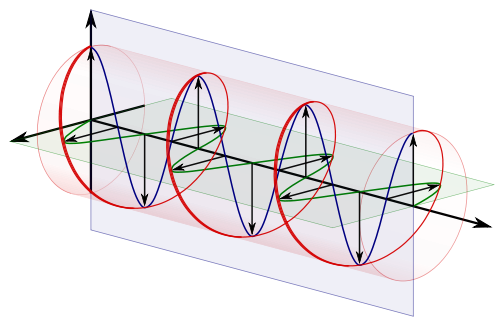
\includegraphics[width=65mm]{Circular.Polarization.png}
\caption{Δεξιόστροφα κυκλικά πολωμένο φως}
\end{figure}
\newpage
\subsubsection {Εφαρμογές}
\begin{description}
  \item[FM Radio] \hfill \\
Ο όρος κυκλική πόλωση χρησιμοποιείται πολύ συχνά για να περιγράψει μικτά πολωμένα σήματα τα οποία χρησιμοποιούνται κυρίως στο FM ράδιο (87.5 to 108.0 MHz), όπου μία κάθετη και μία οριζόντια συνιστώσα διαδίδονται ταυτόχρονα απο μία μονή ή συνδιαστική κεραία. Αυτό έχει ως αποτέλεσμα να παράγεται μεγαλύτερη διείσδυση σε κτίρια και περιοχές με χαμηλή λήψη εκπομπής παρά αν χρησιμοποιούσαμε μόνο ένα επίπεδο πόλωσης.
  \item[3D Movies] \hfill \\
Για να παρουσιαστεί μία στερεοσκοπική κινηματογραφική ταινία, δύο εικόνες προβάλλονται υπερθετικά πάνω στην ίδια οθόνη μέσω διαφορετικών πολωτικών φίλτρων. Ο θεατής φοράει χαμηλού κόστους γυαλιά τα οποία επίσης περιέχουν ένα ζευγάρι πολωτικών φίλτρων κατευθυνόμενα διαφορετικα (δεξιόστροφα/αριστερόστροφα με κυκλική πόλωση ή σε γωνίες $90\degrees$, συνήθως $45\degrees$ και $135\degrees$, με γραμμική πόλωση). Καθώς κάθε φίλτρο αφήνει να περάσει μόνο το φως το οποίο είναι ίδια πολωμένο και το μπλοκάρει σε διαφορετική περίπτωση, κάθε μάτι βλέπει διαφορετική εικόνα. Αυτό χρησιμοποιείται για να παραχθεί ένα τρισδιάστατο φαινόμενο προβάλοντας την ίδια σκηνή και στα δύο μάτια, αλλά απεικονιζόμενες από διαφορετική σκοπιά.
\begin{figure} [hb!]
\centering
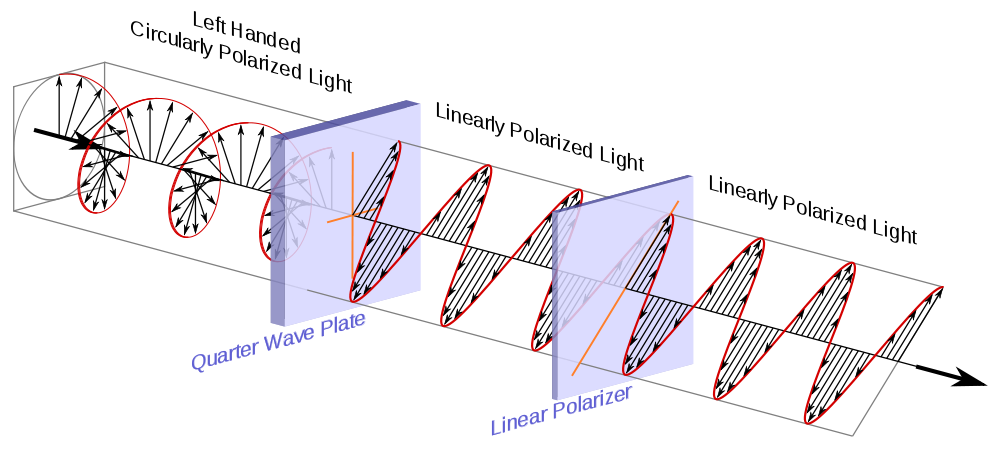
\includegraphics[width=120mm]{3dglasses.png}
\caption{Κυκλικός πολωτής από τον οποίο περνάει αριστερόστροφα κυκλικά πολωμένο φως}
\end{figure}
\end{description}
\newpage

\subsection{Εφαρμογές του ηλεκτροοπτικού φαινομένου  Pockels}

\begin{description}
\item[Ηλεκτροοπτικός διαμορφωτής] \hfill \\
Ένας ηλεκτροοπτικός διαμορφωτής (electro-optic modulator (EOM)) είναι μία συσκευή που μπορεί να χρησιμοποιηθεί για τον έλεγχο της ισχύς, φάσης ή πόλωσης μιας δέσμης laser. Συνήθως περιέχει μία ή δύο κυψελίδες Pockels και πιθανόν πρόσθετα οπτικά στοιχεία όπως πολωτές.

\item[Ηλεκτροοπτική δειγματοληψία] \hfill \\
Η ηλεκτροοπτική δειγματοληψία είναι μία οπτοηλεκτρονική τεχνική οπτικής δειγματοληψίας, η οποία εκμεταλεύεται το διαμήκες ηλεκτροοπτικό φαινόμενο. Όταν υπερβραχείς οπτικοί παλμοί χρησιμοποιούνται σε ηλεκτροοπτικό σωλήνα, υπάρχει μόνο ένα μικρό χρονικό διάστημα στο οποίο το ηλεκτρικό πεδίο στο σωλήνα μπορεί να επηρρεάσει το φως. Αυτό το φαινόμενο - συνήθως μία αλλαγή στην πόλωση, η οποία μετατρέπεται οπτική ισχύ σε έναν πολωτή - μπορεί μετά να μετρηθεί χωρίς να απαιτείται κάποιος πολύ γρήγορος φωτοανιχνευτής.

\item[Ηλεκτροοπτικός διακόπτης] \hfill \\
Μία κυψελίδα Pockels, συνδυασμένη με ένα πολωτή, μπορεί να χρησιμοποιηθεί ως ηλεκτροοπτικός φωτοφράκτης υψηλής ταχύτητας  και είναι συνήθως το ενεργό στοιχείο στα laser ηλεκτροοπτικά παραγόμενου Q. \\Η Q-switching, γνωστή και ως γιγάντια διάταξη παλμού, είναι μία τεχνική με την οποία ένα laser μπορεί να παράγει παλμική δέσμη. Αυτή η τεχνική επιτρέπει την παραγωγή φωτεινών παλμών με εξαιρετικά υψηλή (GW) ισχύ, πολύ περισσότερη από ότι αν το ίδιο laser λειτουργούσε σε συνεχή κλίμακα.
\end{description}


\newpage
\section{Πείραμα}
\subsection{Εισαγωγή}
H διάταξη που χρησιμοποιήθηκε στην άσκηση απεικονίζεται στο παρακάτω σχήμα. 
\begin{figure} [hp]
\centering
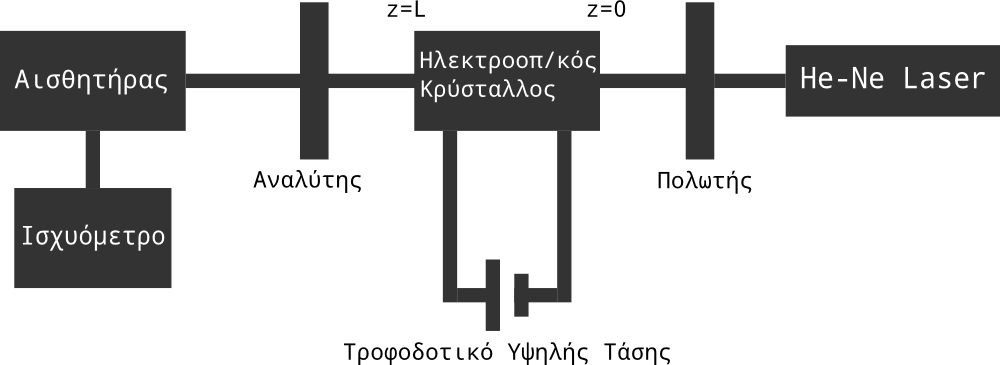
\includegraphics[width=120mm]{diataksh.png}
\caption{Πειραματική διάταξη}
\end{figure}

Το πεδίο του Η/Μ κύματος στο επίπεδο $z=0$, όταν εφαρμόζεται τάση στον ηλεκτροοπτικό κρύσταλλο, αναλύεται σε 2 συνιστώσες κάθετες μεταξύ τους (Σχήμα 5) και πολωμένες στους άξονες $x'$, $y'$. Οι άξονες $x'$, $y'$ προκύπτουν από τους άξονες $x$ και $y$ κατόπιν περιστροφής κατά γωνία $45\degrees$ περί τον άξονα $z$.

\begin{figure} [hp]
\centering
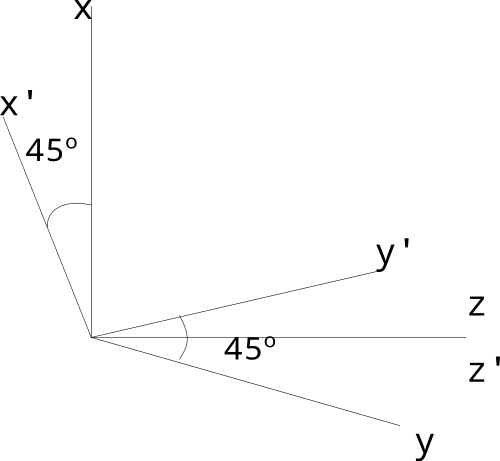
\includegraphics[width=60mm]{aksones.png}
\caption{Πεδίο του Η/Μ κύματος στο επίπεδο $z=0$, όταν εφαρμόζεται τάση στον ηλεκτροοπτικό κρύσταλλο.}
\end{figure}

Ο πολωτής έχει τη δυνατότητα να περιστρέφεται γύρω από τον άξονα $z$ και έχει αριθμημένη κλίμακα γωνίας περιστροφής από $0\degrees - 180\degrees$. Περιστρέφοντας τον πολωτή μεταβάλουμε το επίπεδο πόλωσης της δέσμης που εξέρχεται από τον πολωτή και προσπίπτει στον κρύσταλλο. Συνεπώς αλλάζουμε και τη γωνία που σχηματίζει το διάνυσμα της πόλωσης με τους άξονες $x'$ και $y'$. Επομένως, στην περιοχή τιμών της γωνίας περιστροφής του πολωτή, θα υπάρχουν δύο τιμές που αντιστοιχούν σε γωνία $45\degrees$ μεταξύ του διανύσματος πόλωσης και των αξόνων $x'$ και $y'$ του κρυστάλλου. Όταν ο πολωτής είναι στραμμένος κατά μία απο αυτές τις δύο τιμές της γωνίας περιστροφής τότε η προσπίπτουσα στον κρύσταλλό δέσμη είναι γραμμικά πολωμένη με επίπεδο πόλωσης σε γωνία $45\degrees$ ως προς τους άξονες $x'$ και $y'$. 
\newpage
Ως σφάλματα θεωρήσαμε:

\begin{itemize}
\item $1\degrees$ για τις μετρήσεις του γωνιομέτρου του αναλυτή.
\item $5 mV$ για τις μετρήσεις του ισχυομέτρου (δεν επιλέξαμε 1, επειδή η ένδειξη ήταν αρκετά ευαίσθητη).
\item $0.1 V$ για την υψηλή τάση.
\end{itemize}

Η ένταση του υποβάθρου του διάχυτου φωτός όταν το laser δε λειτουργεί είναι $240mV$.

\subsection{Εύρεση βέλτιστης γωνίας όπου εμφανίζεται κυκλικά πολωμένο φως}
Ξεκινήσαμε το πείραμα εφαρμόζοντας στον κρύσταλλο τάση $V_{\lambda /4}$ ($1500 V$)έτσι ώστε η εξερχόμενη από τον κρύσταλλο δέσμη να είναι κυκλικά πολωμένη. Αυτό το διαπιστώνουμε με τη γωνία του αναλύτη, ο οποίος έχει επίσης τη δυνατότητα περιστροφής και στον οποίο προσπίπτει η εξερχόμενη από τον κρύσταλλο δέσμη, προσπίπτοντας ακολούθως στον αισθητήρα του ισχυομέτρου. 
Τα βήματα που ακολουθήσαμε είναι τα εξής:
\begin{itemize}
\item Περιστρέφαμε τον πολωτή από τις $0\degrees$  και με βήμα $10\degrees$ φτάσαμε ως τις $80\degrees$.
\item Σε κάθε βήμα του πολωτή περιστρέφαμε τον αναλυτή αργά από $0\degrees - 180\degrees$ καταγράφοντας παράλληλα τη μέγιστη και ελάχιστη ένδειξη του ισχυομέτρου.
\end{itemize}
Με αυτό τον τρόπο βρίσκουμε τη γωνία του πολωτή στην οποία εμφανίζεται το πλησιέστερο προς την κυκλική πόλωση ελλειπτικά πολωμένο φως. Αυτό θα είναι εκείνο για το οποίο η διαφορά μεταξύ της ελάχιστης και μέγιστης τιμής της εξερχόμενης έντασης από τον αναλυτή είναι ελάχιστη (Πίνακας 1).

\begin{table} [H]
\centering
\begin{tabular}{|c|c|c|c|}
\hline \rule[-2ex]{0pt}{5.5ex} $Degrees$ Πολωτή & $V_{max} (mV)$ & $V_{min} (mV)$ & $\Delta V (mV)$ \\ 
\hline \rule[-2ex]{0pt}{5.5ex} 0 & 396 & 261 & 134 \\
\hline \rule[-2ex]{0pt}{5.5ex} 10 & 398 & 265 & 129 \\
\hline \rule[-2ex]{0pt}{5.5ex} 20 & 393 & 312 & 81 \\
\hline \rule[-2ex]{0pt}{5.5ex} 30 & 390 & 230 & 60 \\
\hline \rule[-2ex]{0pt}{5.5ex} 40 & 388 & 346 & 42 \\
\hline \rule[-2ex]{0pt}{5.5ex} 50 & 385 & 352 & 33 \\
\hline \rule[-2ex]{0pt}{5.5ex} 60 & 389 & 346 & 43 \\
\hline \rule[-2ex]{0pt}{5.5ex} 70 & 392 & 329 & 63\\
\hline \rule[-2ex]{0pt}{5.5ex} 80 & 396 & 305 & 91 \\
\hline 
\end{tabular} 
\caption{Γωνία του πολωτή στην οποία εμφανίζεται το πλησιέστερο προς την κυκλική πόλωση ελλειπτικά πολωμένο φως.}
\end{table}


\newpage

Έπειτα επαναλάβαμε τα παραπάνω βήματα για την ελάχιστη γωνία που βρήκαμε στον Πίνακα 1 ($50\degrees$), με εύρος $\pm 5\degrees$ ώστε να βελτιστοποιήσουμε τη γωνία που ψάχνουμε. Τα αποτελέσματα εμφανίζονται στον Πίνακα 2.

\begin{table} [H]
\centering
\begin{tabular}{|c|c|c|c|}
\hline \rule[-2ex]{0pt}{5.5ex} $Degrees$ Πολωτή & $V_{max} (mV)$ & $V_{min} (mV)$ & $\Delta V (mV)$ \\ 
\hline \rule[-2ex]{0pt}{5.5ex} 45 & 384 & 353 & 31 \\ 
\hline \rule[-2ex]{0pt}{5.5ex} 46 & 383 & 352 & 31 \\ 
\hline \rule[-2ex]{0pt}{5.5ex} 47 & 383 & 353 & 30 \\ 
\hline \rule[-2ex]{0pt}{5.5ex} 48 & 383 & 353 & 30 \\ 
\hline \rule[-2ex]{0pt}{5.5ex} 49 & 383 & 353 & 30 \\ 
\hline \rule[-2ex]{0pt}{5.5ex} 50 & 383 & 352 & 31 \\ 
\hline \rule[-2ex]{0pt}{5.5ex} 51 & 383 & 354 & 29 \\ 
\hline \rule[-2ex]{0pt}{5.5ex} 52 & 383 & 351 & 32 \\ 
\hline \rule[-2ex]{0pt}{5.5ex} 53 & 383 & 350 & 33 \\ 
\hline \rule[-2ex]{0pt}{5.5ex} 54 & 385 & 350 & 35 \\ 
\hline \rule[-2ex]{0pt}{5.5ex} 55 & 385 & 350 & 35 \\ 
\hline 
\end{tabular} 
\caption{Βελτιστοποίηση γωνίας του πολωτή στην οποία εμφανίζεται το πλησιέστερο προς την κυκλική πόλωση ελλειπτικά πολωμένο φως.}
\end{table}

\subsection{Εύρεση τάσης $V_{\lambda/4}$}

Η γωνία που βρήκαμε στο παραπάνω βήμα ($51\degrees$) (όπου η διαφορά μεταξύ της ελάχιστης και μέγιστης τιμής της εξερχόμενης έντασης από τον αναλυτή είναι ελάχιστη) είναι εκείνη στην οποία πρέπει να στραφεί ο πολωτής ώστε να δημιουργηθεί στην έξοδο του κρυστάλλου δέσμη πλησιέστερη προς \textit{κυκλικά πολωμένη} δέσμη. H γωνία αυτή, είναι εκείνη που δημιουργεί πόλωση της δέσμης του laser \textit{παράλληλη} στον διηλεκτρικό άξονα $x$ του κρυστάλλου, όταν δεν εφαρμόζεται τάση. Έχοντας λοιπόν σταθερό τον πολωτή στις $51\degrees$, τα βήματα που ακολουθήσαμε ήταν τα εξής:
\begin{itemize}
\item Ξεκινήσαμε από τα $500 V$ και με βήμα $100$ φτάσαμε ως τα $2000 V$.
\item Σε κάθε βήμα ψάχναμε στον αναλυτή τη μέγιστη και ελάχιστη γωνία.
\item Σε κάθε μέγιστη και ελάχιστη γωνία καταγράφαμε την ένταση της εξερχόμενης από τον αναλυτή δέσμης.
\end{itemize}

Τα αποτελέσματα εμφανίζονται στον παρακάτω πίνακα.
\newpage
\begin{table} [!hbp]
\centering
\begin{tabular}{|c|c|c|c|}
\hline \rule[-2ex]{0pt}{5.5ex} $High Voltage (V)$ & $V_{max} (mV)$ & $V_{min} (mV)$ & $\Delta V (mV)$ \\ 
\hline \rule[-2ex]{0pt}{5.5ex} 500 & 385 & 342 & 43 \\ 
\hline \rule[-2ex]{0pt}{5.5ex} 600 & 383 & 345 & 38 \\ 
\hline \rule[-2ex]{0pt}{5.5ex} 700 & 380 & 351 & 27\\ 
\hline \rule[-2ex]{0pt}{5.5ex} 800 & 380 & 353 & 27 \\ 
\hline \rule[-2ex]{0pt}{5.5ex} 900 & 376 & 359 & 17 \\ 
\hline \rule[-2ex]{0pt}{5.5ex} 1000 & 375 & 361 & 14 \\ 
\hline \rule[-2ex]{0pt}{5.5ex} 1100 & 374 & 362 & 12 \\ 
\hline \rule[-2ex]{0pt}{5.5ex} 1200 & 370 & 364 & 6 \\ 
\hline \rule[-2ex]{0pt}{5.5ex} 1300 & 369 & 364 & 5 \\ 
\hline \rule[-2ex]{0pt}{5.5ex} 1400 & 372 & 362 & 10 \\ 
\hline \rule[-2ex]{0pt}{5.5ex} 1500 & 374 & 360 & 14 \\ 
\hline \rule[-2ex]{0pt}{5.5ex} 1600 & 376 & 358 & 18 \\ 
\hline \rule[-2ex]{0pt}{5.5ex} 1700 & 378 & 355 & 23 \\ 
\hline \rule[-2ex]{0pt}{5.5ex} 1800 & 380 & 349 & 31 \\ 
\hline \rule[-2ex]{0pt}{5.5ex} 1900 & 382 & 345 & 37 \\ 
\hline \rule[-2ex]{0pt}{5.5ex} 2000 & 382 & 345 & 37 \\ 
\hline 
\end{tabular} 
\caption{Τάση $V_{\lambda/4}$ στην οποία εμφανίζεται το πλησιέστερο προς την κυκλική πόλωση ελλειπτικά πολωμένο φως.}
\end{table}

Παρατηρούμε πως στην περιοχή 1200-1400 $V$ η διαφορά των τάσεων μεταξύ μέγιστης και ελάχιστης τιμής του ισχυομέτρου είναι η ελάχιστη, οπότε σε αυτό το εύρος βρήκαμε την  πειραματική $V_{\lambda/4}$. Η αναμενόμενη τιμή είναι περίπου στα 1500 $V$. Η απόκλιση της πειραματικής τιμής από τη θεωρητική μπορεί να οφείλεται σε παράγοντες όπως η ακτινοβολία του υποβάθρου φωτός καθώς και στην ένδειξη του ισχυόμετρου το οποίο ήταν ευαίσθητο και συνεπώς όχι τόσο σταθερό όταν παίρναμε τις μετρήσεις. 
\\\\
Παρακάτω παρατίθενται οι γραφικές παραστάσεις των πειραματικών δεδομένων.

\begin{figure} [hp!]
\centering
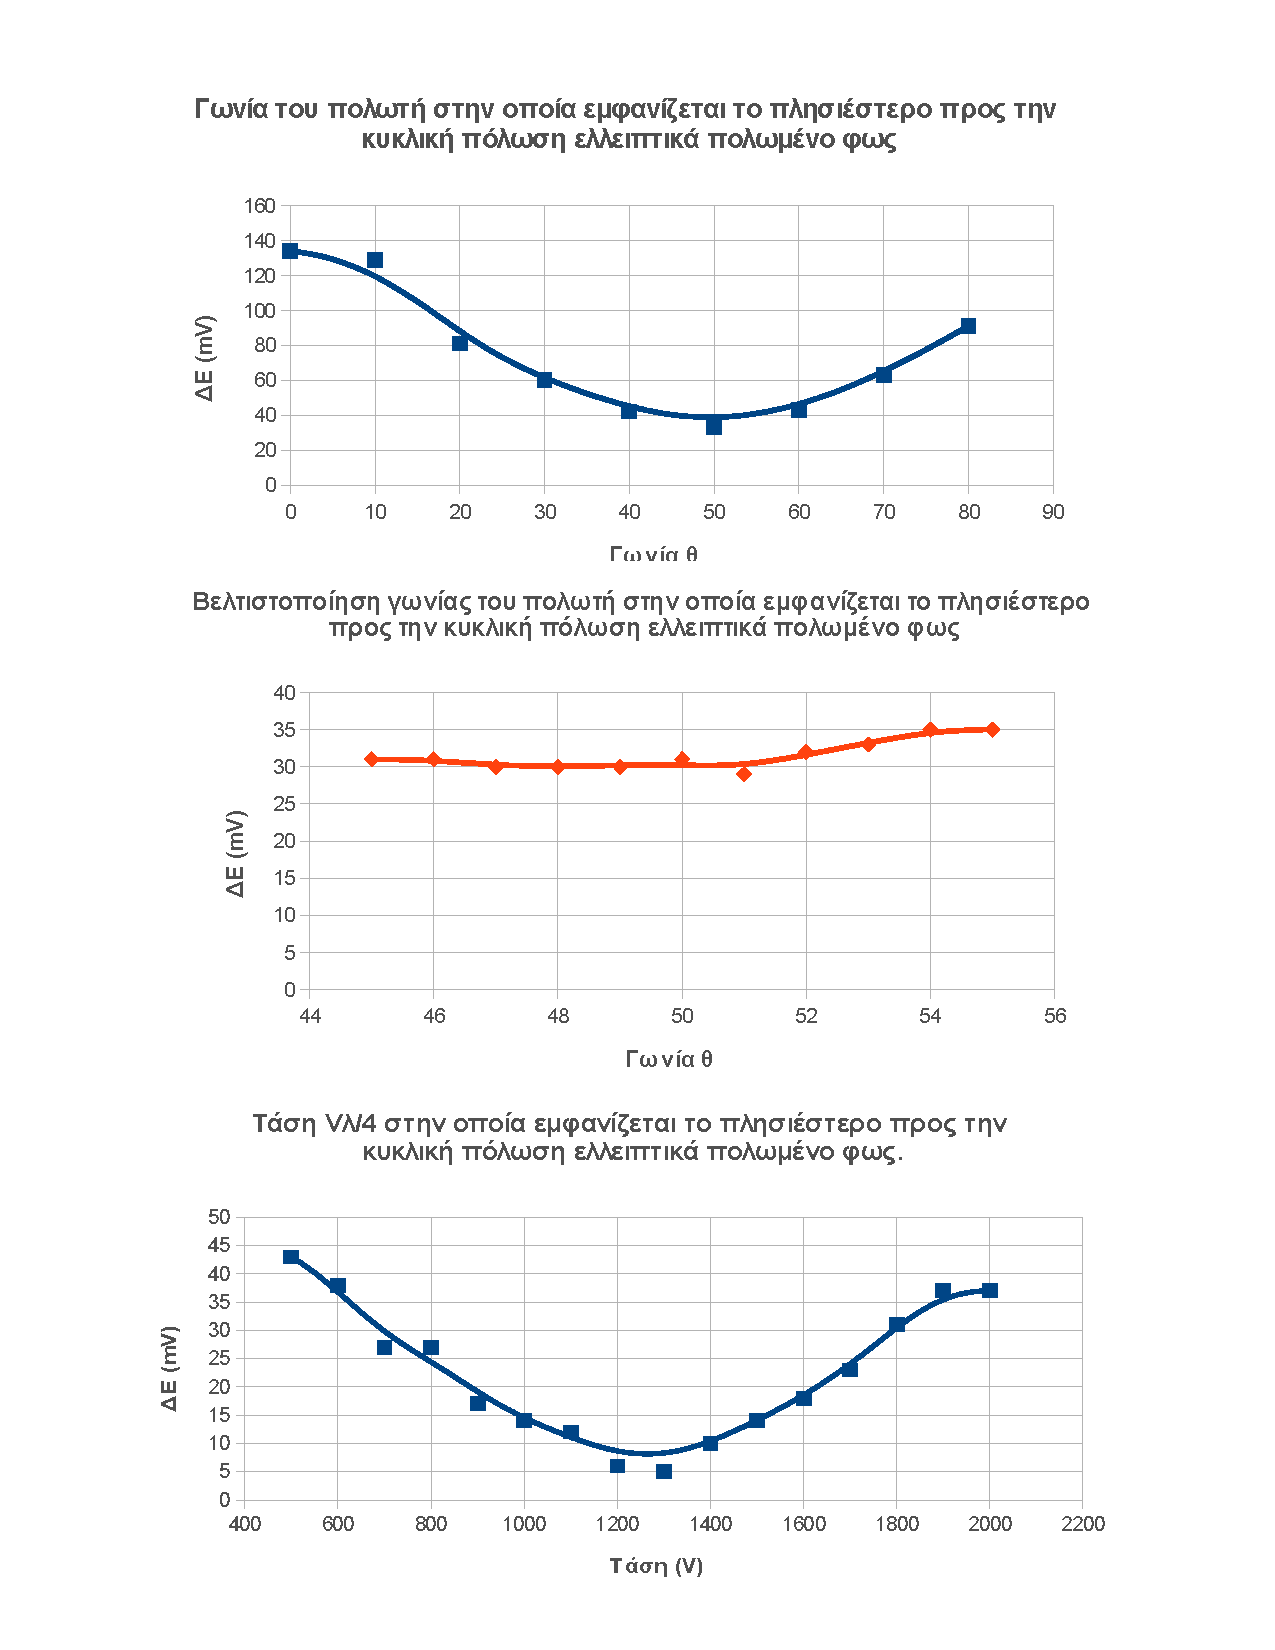
\includegraphics[width=180mm]{tables.pdf}
\end{figure}

\newpage

\begin{thebibliography}{9}

\bibitem{wikipedia}  Wikipedia: Pockels effect, Circular polarization, Birefringence, Q-switching
\bibitem{rp-photonics.com} Encyclopedia of Laser Physics and Technology, www.rp-photonics.com
\bibitem{semfe} Εργαστηριακές Ασκήσεις Οπτοηλεκτρονικής - Φυσικής και τεχνολογίας των Lasers, ΕΜΠ ΣΕΜΦΕ Τομέας Φυσικής, Αθήνα 2005
\bibitem{Young}  Hugh D. Young, Ηλεκτρομαγνητισμός - Οπτική - Σύγχρονη Φυσική, Εκδόσεις Παπαζήση, 8η έκδοση 1994 
\bibitem{M.Young} Matt Young, Οπτική και Λέιζερ, Εκδόσεις ΕΜΠ, 2η έκδοση 2008 

\end{thebibliography}


\end{document}